\documentclass[journal, onecolumn]{IEEEtran}

% --- PACKAGES ---
\usepackage{amsmath}
\usepackage{amssymb}
\usepackage{amsfonts}
\usepackage{amsthm}
\usepackage{graphicx}
\usepackage[utf8]{inputenc}
\usepackage[T1]{fontenc}
\usepackage{url}
\usepackage{xcolor}
\usepackage{enumitem}
\usepackage{tcolorbox}
\usepackage{tikz}
\usepackage{float}
\usepackage{booktabs}
\usepackage{multirow}
\usepackage[normalem]{ulem}
\usetikzlibrary{arrows.meta, positioning, shapes.geometric, calc, decorations.pathreplacing}

% --- USER PREFERENCE COLORS ---
\definecolor{Garnet}{HTML}{73000a}
\definecolor{SecondaryBlue}{HTML}{466A9F}
\definecolor{SecondaryGreen}{HTML}{65780B}
\definecolor{FlatRed}{HTML}{CC2E40}
\definecolor{FlatDark}{HTML}{1F414D}
\definecolor{FlatYellow}{HTML}{CED318}
\definecolor{FlatGold}{HTML}{A49137}
\definecolor{LightGray}{HTML}{F0F0F0}
\definecolor{Rose}{HTML}{CC2E40}

% --- FORMATTING ---
\setlength{\parindent}{0pt}
\setlength{\parskip}{1.2em}
\renewcommand{\baselinestretch}{1.2}

% --- CUSTOM COMMANDS ---
\newcommand{\vocab}[1]{\textbf{\textcolor{Garnet}{#1}}}
\newcommand{\mathhighlight}[1]{\textcolor{SecondaryBlue}{#1}}

% --- TCOLORBOX STYLES ---
\tcbset{
    examplebox/.style={
        colback=LightGray,
        colframe=SecondaryBlue,
        fonttitle=\bfseries,
        title=#1,
        sharp corners,
        boxrule=1pt
    },
    memorybox/.style={
        colback=Garnet!10,
        colframe=Garnet,
        fonttitle=\bfseries,
        title=#1,
        sharp corners,
        boxrule=2pt
    }
}

% --- TITLE & AUTHOR ---
\title{\textcolor{Garnet}{\textbf{Monte Carlo Prediction: First-Visit vs Every-Visit}}\\[0.3em]
\large A Visual Guide with Worked Examples}
\author{CSCE 775 -- Reinforcement Learning}
\date{\today}

\begin{document}
\maketitle

% ============================================================
\section{Introduction}
% ============================================================

In reinforcement learning, one of the most fundamental questions is: ``How good is it to be in a particular state?'' We answer this by estimating the \vocab{value function} $V(s)$, which tells us the total reward we can expect to collect starting from state $s$ if we follow a particular policy (i.e., a particular strategy for choosing actions). A high value means the state is a good place to be; a low or negative value means things are likely to go poorly from there.

\subsection{Two Approaches: Dynamic Programming vs Monte Carlo}

There are two major families of methods for estimating $V(s)$.

\vocab{Dynamic Programming (DP)} uses the Bellman equation to compute $V(s)$ by looking at all the states we \textit{could} transition to, weighted by their probabilities. This requires a \vocab{model} of the environment, meaning we need to know two things exactly. First, the \textit{transition probabilities} $p(s' \mid s, a)$, which answer the question ``if I'm in state $s$ and take action $a$, what is the probability I end up in state $s'$?'' Second, the \textit{reward function} $r(s, a, s')$, which tells us the reward for each transition. If we have these, DP can compute the value function precisely without ever actually interacting with the environment.

The problem is that in many real-world situations, we \textit{do not} have this model. Consider a robot navigating a warehouse, or an agent playing a video game. We might not know the exact probabilities of what happens next. We only know what \textit{actually happened} when we tried things.

\vocab{Monte Carlo (MC) prediction} takes a completely different approach. Instead of computing values from a model, MC methods learn directly from \vocab{experience}. We let the agent interact with the environment, collect complete episodes (sequences of states, actions, and rewards from start to finish), and then estimate $V(s)$ by averaging the actual rewards we observed. This is what it means to be \vocab{model-free}: we do not need to know $p(s' \mid s, a)$ or $r(s, a, s')$ at all. We just need to be able to generate episodes by running the policy.

\begin{tcolorbox}[examplebox={When to Use Which?}]
\textbf{Use Dynamic Programming} when you have a complete, accurate model of the environment (transition probabilities and rewards). DP is exact and efficient for small, well-defined problems like simple gridworlds where all the rules are known.

\textbf{Use Monte Carlo methods} when you do not have a model, or the model is too complex to use. MC only requires the ability to generate sample episodes. This makes MC applicable to situations like games, robotics, or any setting where you can simulate or interact with the environment but cannot write down all the transition probabilities.
\end{tcolorbox}

\subsection{The Core Idea}

The value of a state under a policy $\pi$ is defined as the \textit{expected return} starting from that state.
\begin{align}
    V^\pi(s) = \mathbb{E}_\pi\left[G_t \mid S_t = s\right]
\end{align}
Let us unpack each piece of notation. $V^\pi(s)$ is the value of state $s$ when following policy $\pi$. The symbol $\mathbb{E}_\pi[\cdot]$ means ``the expected value (average) if we follow policy $\pi$.'' The term $G_t$ is the \vocab{return} at time step $t$, which is the total discounted reward from time $t$ onward (we will compute this explicitly in Section~IV). The expression $S_t = s$ means ``given that we are in state $s$ at time $t$.'' Putting it together, Equation (1) says: the value of state $s$ is the average total reward we would get, starting from $s$ and following our policy.

MC prediction approximates this expected value by collecting actual returns $G_t$ from many episodes and computing their \textit{sample mean} (just a plain average). The two most common variants, \vocab{first-visit MC} and \vocab{every-visit MC}, differ in how they handle states that appear more than once in a single episode. The rest of this guide walks through a concrete example to make this difference crystal clear.

% ============================================================
\section{The Gridworld}
% ============================================================

Consider the following $3 \times 3$ gridworld with states $S_1$ through $S_9$. The agent can move in the four cardinal directions. State $S_9$ is the \vocab{terminal state} (goal). Stepping into the goal yields a reward of $R = +10$, while every other step yields $R = -1$. The discount factor is $\gamma = 0.9$.

\begin{figure}[H]
\centering
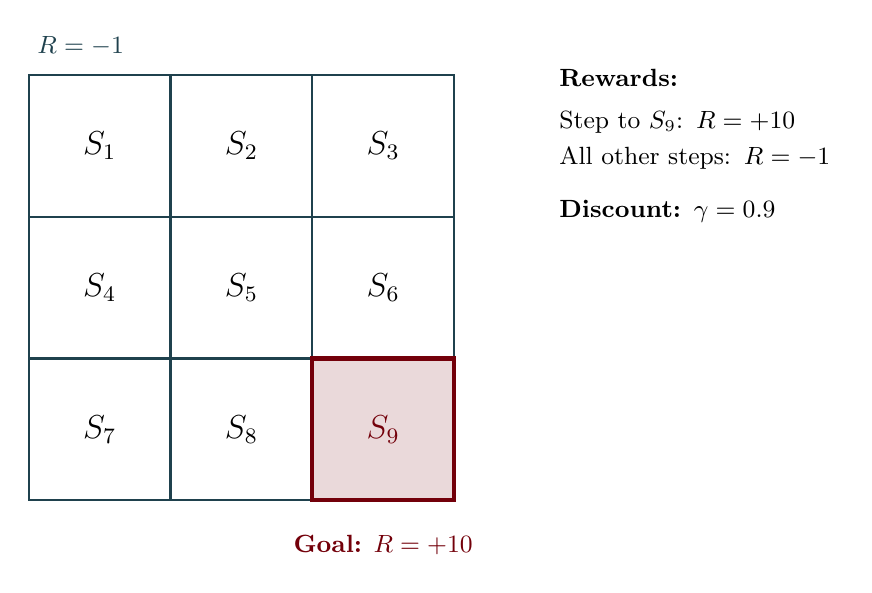
\begin{tikzpicture}[
    cell/.style={minimum size=1.8cm, draw=FlatDark, thick, font=\large},
    goal/.style={cell, fill=Garnet!15, draw=Garnet, line width=1.5pt},
    rlabel/.style={font=\small, FlatDark}
]
% Row 1 (top): S1, S2, S3
\node[cell] (s1) at (0, 3.6) {$S_1$};
\node[cell] (s2) at (1.8, 3.6) {$S_2$};
\node[cell] (s3) at (3.6, 3.6) {$S_3$};
% Row 2: S4, S5, S6
\node[cell] (s4) at (0, 1.8) {$S_4$};
\node[cell] (s5) at (1.8, 1.8) {$S_5$};
\node[cell] (s6) at (3.6, 1.8) {$S_6$};
% Row 3 (bottom): S7, S8, S9
\node[cell] (s7) at (0, 0) {$S_7$};
\node[cell] (s8) at (1.8, 0) {$S_8$};
\node[goal] (s9) at (3.6, 0) {\textcolor{Garnet}{$S_9$}};

% Reward labels
\node[rlabel, above=0.1cm of s1.north west, anchor=south west] {$R = -1$};
\node[rlabel, below=0.3cm of s9] {\textcolor{Garnet}{\textbf{Goal:} $R = +10$}};

% Legend
\node[right=1.2cm of s3, anchor=west, font=\small, text width=3.5cm] {
    \textbf{Rewards:}\\[2pt]
    Step to $S_9$: $R = +10$\\
    All other steps: $R = -1$\\[6pt]
    \textbf{Discount:} $\gamma = 0.9$
};
\end{tikzpicture}
\caption{The $3\times 3$ gridworld. $S_9$ (garnet) is the terminal goal state.}
\label{fig:gridworld}
\end{figure}

% ============================================================
\section{A Sample Episode}
% ============================================================

Suppose the agent follows its policy and generates the following episode. Notice that the agent revisits states $S_1$ and $S_2$, which is exactly the scenario where first-visit and every-visit MC differ.

\begin{tcolorbox}[examplebox={Episode Trajectory}]
$S_1 \xrightarrow{-1} S_2 \xrightarrow{-1} S_5 \xrightarrow{-1} S_4 \xrightarrow{-1}
\textcolor{Rose}{S_1} \xrightarrow{-1} \textcolor{Rose}{S_2} \xrightarrow{-1} S_3 \xrightarrow{-1} S_6 \xrightarrow{+10} S_9$

\medskip
States shown in \textcolor{Rose}{\textbf{rose}} are \textit{revisits}, i.e., the agent has already visited them earlier in the episode.
\end{tcolorbox}

The following diagram traces this path on the gridworld. Each arrow is numbered by its time step, and revisited transitions are drawn in \textcolor{Rose}{rose}.

\begin{figure}[H]
\centering
\begin{tikzpicture}[
    cell/.style={minimum size=1.8cm, draw=FlatDark!40, thick, font=\large},
    goal/.style={cell, fill=Garnet!15, draw=Garnet, line width=1.5pt},
    arr/.style={-{Stealth[length=3mm]}, line width=1.2pt, FlatDark},
    revisit/.style={-{Stealth[length=3mm]}, line width=1.2pt, Rose},
    step/.style={font=\scriptsize\bfseries, fill=white, inner sep=1pt},
    rstep/.style={font=\scriptsize\bfseries, fill=white, inner sep=1pt, Rose}
]
% Grid
\node[cell] (s1) at (0, 3.6) {$S_1$};
\node[cell] (s2) at (1.8, 3.6) {$S_2$};
\node[cell] (s3) at (3.6, 3.6) {$S_3$};
\node[cell] (s4) at (0, 1.8) {$S_4$};
\node[cell] (s5) at (1.8, 1.8) {$S_5$};
\node[cell] (s6) at (3.6, 1.8) {$S_6$};
\node[cell] (s7) at (0, 0) {$S_7$};
\node[cell] (s8) at (1.8, 0) {$S_8$};
\node[goal] (s9) at (3.6, 0) {\textcolor{Garnet}{$S_9$}};

% Arrows with step numbers
% Step 0: S1 -> S2
\draw[arr] ([yshift=2pt]s1.east) -- ([yshift=2pt]s2.west) node[step, midway, above=1pt] {0};
% Step 1: S2 -> S5
\draw[arr] ([xshift=-2pt]s2.south) -- ([xshift=-2pt]s5.north) node[step, midway, left=1pt] {1};
% Step 2: S5 -> S4
\draw[arr] ([yshift=-2pt]s5.west) -- ([yshift=-2pt]s4.east) node[step, midway, below=1pt] {2};
% Step 3: S4 -> S1
\draw[arr] ([xshift=2pt]s4.north) -- ([xshift=2pt]s1.south) node[step, midway, right=1pt] {3};
% Step 4: S1 -> S2 (revisit)
\draw[revisit] ([yshift=-2pt]s1.east) -- ([yshift=-2pt]s2.west) node[rstep, midway, below=1pt] {4};
% Step 5: S2 -> S3 (revisit of S2)
\draw[revisit] ([yshift=2pt]s2.east) -- ([yshift=2pt]s3.west) node[rstep, midway, above=1pt] {5};
% Step 6: S3 -> S6
\draw[arr] ([xshift=2pt]s3.south) -- ([xshift=2pt]s6.north) node[step, midway, right=1pt] {6};
% Step 7: S6 -> S9
\draw[arr] ([xshift=2pt]s6.south) -- ([xshift=2pt]s9.north) node[step, midway, right=1pt] {7};

% Start marker
\node[above=0.25cm of s1, font=\small\bfseries, FlatDark] {START};
\end{tikzpicture}
\caption{Episode path on the gridworld. Black arrows show first visits; \textcolor{Rose}{rose arrows} show revisits of $S_1$ and $S_2$.}
\label{fig:episode_path}
\end{figure}

% ============================================================
\section{Computing Returns}
% ============================================================

The return $G_t$ at each time step is computed \textit{backward} from the terminal state using the recursive definition.
\begin{align}
    G_t = R_{t+1} + \gamma \, G_{t+1}
\end{align}
Starting from the final transition at $t = 7$ and working backward gives the following.

\begin{tcolorbox}[examplebox={Backward Return Computation}]
\begin{align}
G_7 &= R_8 = +10 && \text{($S_6 \to S_9$: terminal reward)} \notag\\[4pt]
G_6 &= R_7 + \gamma G_7 = -1 + 0.9(10) = \mathhighlight{8.0} && \text{(at $S_3$)} \notag\\[4pt]
G_5 &= R_6 + \gamma G_6 = -1 + 0.9(8.0) = \mathhighlight{6.2} && \text{(at $S_2$, 2nd visit)} \notag\\[4pt]
G_4 &= R_5 + \gamma G_5 = -1 + 0.9(6.2) = \mathhighlight{4.58} && \text{(at $S_1$, 2nd visit)} \notag\\[4pt]
G_3 &= R_4 + \gamma G_4 = -1 + 0.9(4.58) = \mathhighlight{3.122} && \text{(at $S_4$)} \notag\\[4pt]
G_2 &= R_3 + \gamma G_3 = -1 + 0.9(3.122) = \mathhighlight{1.810} && \text{(at $S_5$)} \notag\\[4pt]
G_1 &= R_2 + \gamma G_2 = -1 + 0.9(1.810) = \mathhighlight{0.629} && \text{(at $S_2$, 1st visit)} \notag\\[4pt]
G_0 &= R_1 + \gamma G_1 = -1 + 0.9(0.629) = \mathhighlight{-0.434} && \text{(at $S_1$, 1st visit)} \notag
\end{align}
\end{tcolorbox}

The summary of all returns is given in Table~\ref{tab:returns}.

\begin{table}[H]
\centering
\caption{Returns $G_t$ for each time step in the episode.}
\label{tab:returns}
\begin{tabular}{cccc}
\toprule
\textbf{Time $t$} & \textbf{State} & \textbf{Return $G_t$} & \textbf{Visit \#} \\
\midrule
0 & $S_1$ & $-0.434$ & 1st \\
1 & $S_2$ & $0.629$  & 1st \\
2 & $S_5$ & $1.810$  & 1st \\
3 & $S_4$ & $3.122$  & 1st \\
4 & \textcolor{Rose}{$S_1$} & \textcolor{Rose}{$4.58$}   & \textcolor{Rose}{2nd} \\
5 & \textcolor{Rose}{$S_2$} & \textcolor{Rose}{$6.2$}    & \textcolor{Rose}{2nd} \\
6 & $S_3$ & $8.0$    & 1st \\
7 & $S_6$ & $10.0$   & 1st \\
\bottomrule
\end{tabular}
\end{table}

% ============================================================
\section{First-Visit Monte Carlo Prediction}
% ============================================================

\begin{tcolorbox}[memorybox={Definition: First-Visit MC}]
For each state $s$ appearing in an episode, record the return $G_t$ only for the \vocab{first time} $s$ is visited in that episode. The value estimate is the average of these first-visit returns across all episodes.
\begin{align}
    V(s) \approx \frac{1}{N(s)} \sum_{i=1}^{N(s)} G_t^{(i)} \quad \text{where each } G_t^{(i)} \text{ is from the first visit to } s \text{ in episode } i
\end{align}
\end{tcolorbox}

In our episode, first-visit MC uses only the returns from $t=0$ and $t=1$ for $S_1$ and $S_2$ respectively, \textit{ignoring} the second visits at $t=4$ and $t=5$.

\begin{tcolorbox}[examplebox={First-Visit MC Pseudocode}]
\texttt{Initialize:} $V(s) \leftarrow 0$, $\text{Returns}(s) \leftarrow$ empty list, for all $s$\\[4pt]
\texttt{For each episode:}\\
\quad Generate episode: $S_0, A_0, R_1, S_1, A_1, R_2, \ldots, S_T$\\
\quad $G \leftarrow 0$\\
\quad \texttt{For} $t = T-1, T-2, \ldots, 0$:\\
\quad\quad $G \leftarrow R_{t+1} + \gamma G$\\
\quad\quad \texttt{If} $S_t$ not in $\{S_0, S_1, \ldots, S_{t-1}\}$: \hfill \textcolor{Garnet}{$\triangleleft$ first visit only}\\
\quad\quad\quad Append $G$ to $\text{Returns}(S_t)$\\
\quad\quad\quad $V(S_t) \leftarrow \text{average}(\text{Returns}(S_t))$
\end{tcolorbox}

The following grid shows the first-visit value estimates after processing this single episode. Second-visit returns are crossed out to emphasize they are discarded.

\begin{figure}[H]
\centering
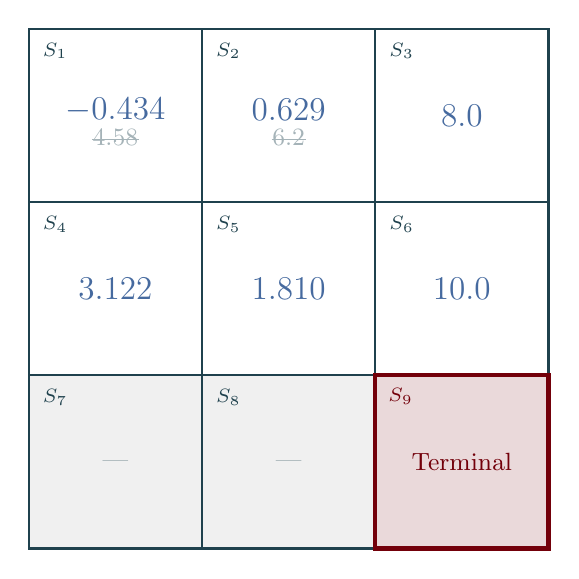
\begin{tikzpicture}[
    cell/.style={minimum size=2.2cm, draw=FlatDark, thick},
    goal/.style={cell, fill=Garnet!15, draw=Garnet, line width=1.5pt},
    empty/.style={cell, fill=LightGray},
    val/.style={font=\large\bfseries, SecondaryBlue},
    struck/.style={font=\small, text=FlatDark!40},
    slabel/.style={font=\scriptsize, FlatDark}
]
% Row 1
\node[cell] (s1) at (0, 4.4) {};
\node[slabel, anchor=north west] at ([shift={(2pt,-2pt)}]s1.north west) {$S_1$};
\node[val] at ([yshift=2pt]s1.center) {$-0.434$};
\node[struck] at ([yshift=-8pt]s1.center) {\sout{$4.58$}};

\node[cell] (s2) at (2.2, 4.4) {};
\node[slabel, anchor=north west] at ([shift={(2pt,-2pt)}]s2.north west) {$S_2$};
\node[val] at ([yshift=2pt]s2.center) {$0.629$};
\node[struck] at ([yshift=-8pt]s2.center) {\sout{$6.2$}};

\node[cell] (s3) at (4.4, 4.4) {};
\node[slabel, anchor=north west] at ([shift={(2pt,-2pt)}]s3.north west) {$S_3$};
\node[val] at (s3.center) {$8.0$};

% Row 2
\node[cell] (s4) at (0, 2.2) {};
\node[slabel, anchor=north west] at ([shift={(2pt,-2pt)}]s4.north west) {$S_4$};
\node[val] at (s4.center) {$3.122$};

\node[cell] (s5) at (2.2, 2.2) {};
\node[slabel, anchor=north west] at ([shift={(2pt,-2pt)}]s5.north west) {$S_5$};
\node[val] at (s5.center) {$1.810$};

\node[cell] (s6) at (4.4, 2.2) {};
\node[slabel, anchor=north west] at ([shift={(2pt,-2pt)}]s6.north west) {$S_6$};
\node[val] at (s6.center) {$10.0$};

% Row 3
\node[empty] (s7) at (0, 0) {};
\node[slabel, anchor=north west] at ([shift={(2pt,-2pt)}]s7.north west) {$S_7$};
\node[font=\small, FlatDark!50] at (s7.center) {---};

\node[empty] (s8) at (2.2, 0) {};
\node[slabel, anchor=north west] at ([shift={(2pt,-2pt)}]s8.north west) {$S_8$};
\node[font=\small, FlatDark!50] at (s8.center) {---};

\node[goal] (s9) at (4.4, 0) {};
\node[slabel, anchor=north west] at ([shift={(2pt,-2pt)}]s9.north west) {\textcolor{Garnet}{$S_9$}};
\node[font=\small, Garnet] at (s9.center) {Terminal};
\end{tikzpicture}
\caption{First-visit MC estimates. \sout{Struck values} are second-visit returns that are discarded.}
\label{fig:first_visit_grid}
\end{figure}

% ============================================================
\section{Every-Visit Monte Carlo Prediction}
% ============================================================

\begin{tcolorbox}[memorybox={Definition: Every-Visit MC}]
For each state $s$ appearing in an episode, record the return $G_t$ for \vocab{every time} $s$ is visited. The value estimate is the average of \textit{all} observed returns for $s$ across all episodes.
\begin{align}
    V(s) \approx \frac{1}{N(s)} \sum_{i=1}^{N(s)} G_t^{(i)} \quad \text{where each } G_t^{(i)} \text{ is from \textit{any} visit to } s
\end{align}
\end{tcolorbox}

Every-visit MC uses \textit{both} returns for $S_1$ and $S_2$.

For $S_1$:
\begin{align}
    V(S_1) = \frac{G_0 + G_4}{2} = \frac{-0.434 + 4.58}{2} = \mathhighlight{2.073}
\end{align}

For $S_2$:
\begin{align}
    V(S_2) = \frac{G_1 + G_5}{2} = \frac{0.629 + 6.2}{2} = \mathhighlight{3.414}
\end{align}

\begin{figure}[H]
\centering
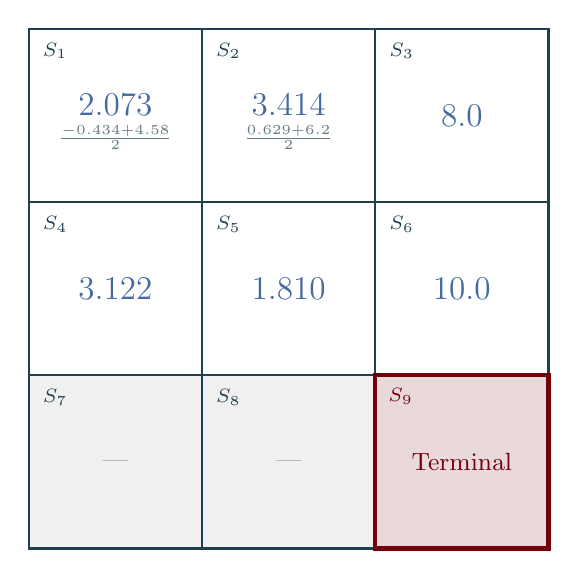
\begin{tikzpicture}[
    cell/.style={minimum size=2.2cm, draw=FlatDark, thick},
    goal/.style={cell, fill=Garnet!15, draw=Garnet, line width=1.5pt},
    empty/.style={cell, fill=LightGray},
    val/.style={font=\large\bfseries, SecondaryBlue},
    detail/.style={font=\scriptsize, FlatDark!70},
    slabel/.style={font=\scriptsize, FlatDark}
]
% Row 1
\node[cell] (s1) at (0, 4.4) {};
\node[slabel, anchor=north west] at ([shift={(2pt,-2pt)}]s1.north west) {$S_1$};
\node[val] at ([yshift=4pt]s1.center) {$2.073$};
\node[detail] at ([yshift=-8pt]s1.center) {$\frac{-0.434 + 4.58}{2}$};

\node[cell] (s2) at (2.2, 4.4) {};
\node[slabel, anchor=north west] at ([shift={(2pt,-2pt)}]s2.north west) {$S_2$};
\node[val] at ([yshift=4pt]s2.center) {$3.414$};
\node[detail] at ([yshift=-8pt]s2.center) {$\frac{0.629 + 6.2}{2}$};

\node[cell] (s3) at (4.4, 4.4) {};
\node[slabel, anchor=north west] at ([shift={(2pt,-2pt)}]s3.north west) {$S_3$};
\node[val] at (s3.center) {$8.0$};

% Row 2
\node[cell] (s4) at (0, 2.2) {};
\node[slabel, anchor=north west] at ([shift={(2pt,-2pt)}]s4.north west) {$S_4$};
\node[val] at (s4.center) {$3.122$};

\node[cell] (s5) at (2.2, 2.2) {};
\node[slabel, anchor=north west] at ([shift={(2pt,-2pt)}]s5.north west) {$S_5$};
\node[val] at (s5.center) {$1.810$};

\node[cell] (s6) at (4.4, 2.2) {};
\node[slabel, anchor=north west] at ([shift={(2pt,-2pt)}]s6.north west) {$S_6$};
\node[val] at (s6.center) {$10.0$};

% Row 3
\node[empty] (s7) at (0, 0) {};
\node[slabel, anchor=north west] at ([shift={(2pt,-2pt)}]s7.north west) {$S_7$};
\node[font=\small, FlatDark!50] at (s7.center) {---};

\node[empty] (s8) at (2.2, 0) {};
\node[slabel, anchor=north west] at ([shift={(2pt,-2pt)}]s8.north west) {$S_8$};
\node[font=\small, FlatDark!50] at (s8.center) {---};

\node[goal] (s9) at (4.4, 0) {};
\node[slabel, anchor=north west] at ([shift={(2pt,-2pt)}]s9.north west) {\textcolor{Garnet}{$S_9$}};
\node[font=\small, Garnet] at (s9.center) {Terminal};
\end{tikzpicture}
\caption{Every-visit MC estimates. Both returns are averaged for $S_1$ and $S_2$.}
\label{fig:every_visit_grid}
\end{figure}

% ============================================================
\section{Side-by-Side Comparison}
% ============================================================

The two grids below place the first-visit and every-visit estimates next to each other. The cells where the estimates differ ($S_1$ and $S_2$) are highlighted in \textcolor{Rose}{rose}.

\begin{figure}[H]
\centering
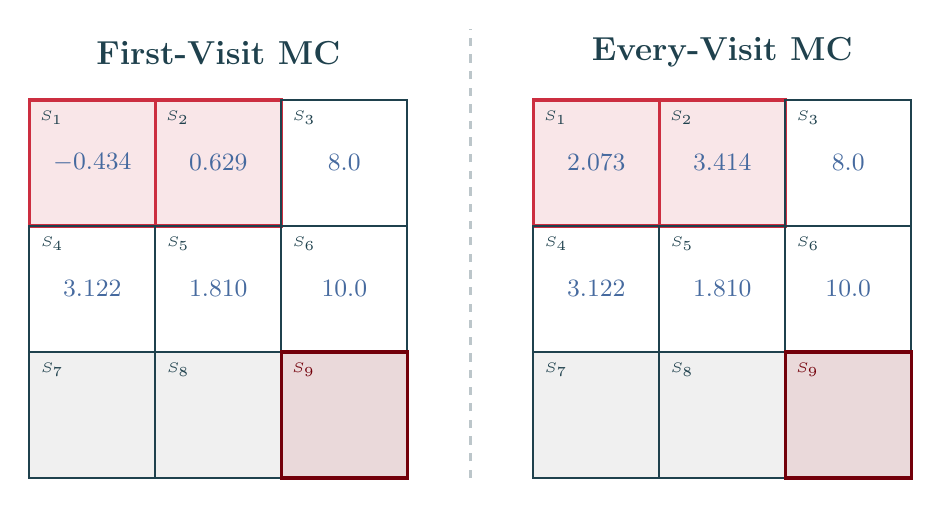
\begin{tikzpicture}[
    cell/.style={minimum size=1.6cm, draw=FlatDark, thick, font=\normalsize},
    diff/.style={cell, fill=Rose!12, draw=Rose, line width=1.2pt},
    goal/.style={cell, fill=Garnet!15, draw=Garnet, line width=1.2pt},
    empty/.style={cell, fill=LightGray},
    val/.style={font=\small\bfseries, SecondaryBlue},
    slabel/.style={font=\tiny, FlatDark},
    heading/.style={font=\large\bfseries, FlatDark}
]

% === First-Visit Grid (left) ===
\node[heading] at (1.6, 6.2) {First-Visit MC};

% Row 1
\node[diff] (fv1) at (0, 4.8) {};
\node[slabel, anchor=north west] at ([shift={(1pt,-1pt)}]fv1.north west) {$S_1$};
\node[val] at (fv1.center) {$-0.434$};

\node[diff] (fv2) at (1.6, 4.8) {};
\node[slabel, anchor=north west] at ([shift={(1pt,-1pt)}]fv2.north west) {$S_2$};
\node[val] at (fv2.center) {$0.629$};

\node[cell] (fv3) at (3.2, 4.8) {};
\node[slabel, anchor=north west] at ([shift={(1pt,-1pt)}]fv3.north west) {$S_3$};
\node[val] at (fv3.center) {$8.0$};

% Row 2
\node[cell] (fv4) at (0, 3.2) {};
\node[slabel, anchor=north west] at ([shift={(1pt,-1pt)}]fv4.north west) {$S_4$};
\node[val] at (fv4.center) {$3.122$};

\node[cell] (fv5) at (1.6, 3.2) {};
\node[slabel, anchor=north west] at ([shift={(1pt,-1pt)}]fv5.north west) {$S_5$};
\node[val] at (fv5.center) {$1.810$};

\node[cell] (fv6) at (3.2, 3.2) {};
\node[slabel, anchor=north west] at ([shift={(1pt,-1pt)}]fv6.north west) {$S_6$};
\node[val] at (fv6.center) {$10.0$};

% Row 3
\node[empty] (fv7) at (0, 1.6) {};
\node[slabel, anchor=north west] at ([shift={(1pt,-1pt)}]fv7.north west) {$S_7$};

\node[empty] (fv8) at (1.6, 1.6) {};
\node[slabel, anchor=north west] at ([shift={(1pt,-1pt)}]fv8.north west) {$S_8$};

\node[goal] (fv9) at (3.2, 1.6) {};
\node[slabel, anchor=north west] at ([shift={(1pt,-1pt)}]fv9.north west) {\textcolor{Garnet}{$S_9$}};

% === Every-Visit Grid (right) ===
\node[heading] at (8.0, 6.2) {Every-Visit MC};

% Row 1
\node[diff] (ev1) at (6.4, 4.8) {};
\node[slabel, anchor=north west] at ([shift={(1pt,-1pt)}]ev1.north west) {$S_1$};
\node[val] at (ev1.center) {$2.073$};

\node[diff] (ev2) at (8.0, 4.8) {};
\node[slabel, anchor=north west] at ([shift={(1pt,-1pt)}]ev2.north west) {$S_2$};
\node[val] at (ev2.center) {$3.414$};

\node[cell] (ev3) at (9.6, 4.8) {};
\node[slabel, anchor=north west] at ([shift={(1pt,-1pt)}]ev3.north west) {$S_3$};
\node[val] at (ev3.center) {$8.0$};

% Row 2
\node[cell] (ev4) at (6.4, 3.2) {};
\node[slabel, anchor=north west] at ([shift={(1pt,-1pt)}]ev4.north west) {$S_4$};
\node[val] at (ev4.center) {$3.122$};

\node[cell] (ev5) at (8.0, 3.2) {};
\node[slabel, anchor=north west] at ([shift={(1pt,-1pt)}]ev5.north west) {$S_5$};
\node[val] at (ev5.center) {$1.810$};

\node[cell] (ev6) at (9.6, 3.2) {};
\node[slabel, anchor=north west] at ([shift={(1pt,-1pt)}]ev6.north west) {$S_6$};
\node[val] at (ev6.center) {$10.0$};

% Row 3
\node[empty] (ev7) at (6.4, 1.6) {};
\node[slabel, anchor=north west] at ([shift={(1pt,-1pt)}]ev7.north west) {$S_7$};

\node[empty] (ev8) at (8.0, 1.6) {};
\node[slabel, anchor=north west] at ([shift={(1pt,-1pt)}]ev8.north west) {$S_8$};

\node[goal] (ev9) at (9.6, 1.6) {};
\node[slabel, anchor=north west] at ([shift={(1pt,-1pt)}]ev9.north west) {\textcolor{Garnet}{$S_9$}};

% Separator
\draw[FlatDark!30, dashed, line width=1pt] (4.8, 0.8) -- (4.8, 6.5);
\end{tikzpicture}
\caption{Side-by-side comparison. Cells highlighted in \textcolor{Rose}{rose} differ between the two methods.}
\label{fig:comparison}
\end{figure}

\begin{table}[H]
\centering
\caption{Numerical comparison of first-visit and every-visit MC estimates.}
\label{tab:comparison}
\begin{tabular}{lccc}
\toprule
\textbf{State} & \textbf{First-Visit $V(s)$} & \textbf{Every-Visit $V(s)$} & \textbf{Difference} \\
\midrule
$S_1$ & $-0.434$ & $2.073$ & \textcolor{Rose}{$+2.507$} \\
$S_2$ & $0.629$  & $3.414$ & \textcolor{Rose}{$+2.785$} \\
$S_3$ & $8.0$    & $8.0$   & $0$ \\
$S_4$ & $3.122$  & $3.122$ & $0$ \\
$S_5$ & $1.810$  & $1.810$ & $0$ \\
$S_6$ & $10.0$   & $10.0$  & $0$ \\
\bottomrule
\end{tabular}
\end{table}

The difference is substantial. First-visit MC gives $V(S_1) = -0.434$ while every-visit MC gives $V(S_1) = 2.073$. This is because the second visit to $S_1$ (at $t=4$) occurs closer to the goal and thus has a much higher return ($G_4 = 4.58$). Every-visit MC includes this optimistic return in its average, pulling the estimate upward.

% ============================================================
\section{Key Takeaways}
% ============================================================

\begin{tcolorbox}[memorybox={Bias and Variance Properties}]
\textbf{First-Visit MC:}
\begin{itemize}[leftmargin=1.5em, itemsep=2pt]
    \item Each return $G_t$ is an \textit{unbiased} estimate of $V^\pi(s)$ because the first visit to $s$ is a fresh sample from the stationary distribution of episodes starting from $s$.
    \item Returns across different episodes are \textit{independent}, which simplifies convergence analysis.
    \item Converges to $V^\pi(s)$ by the strong law of large numbers as the number of episodes $\to \infty$.
\end{itemize}

\medskip

\textbf{Every-Visit MC:}
\begin{itemize}[leftmargin=1.5em, itemsep=2pt]
    \item Technically \textit{biased} for finite samples because returns from multiple visits within the same episode are correlated (later visits depend on the path that led to the revisit).
    \item However, the bias is \textit{asymptotically zero} and every-visit MC is \textit{consistent}, converging to $V^\pi(s)$ as episodes $\to \infty$.
    \item Generally has \textit{lower variance} than first-visit MC because it uses more data points per episode.
    \item Often preferred in practice due to simpler implementation (no need to track which states have been visited).
\end{itemize}
\end{tcolorbox}

\begin{tcolorbox}[examplebox={When Does It Matter?}]
The difference between first-visit and every-visit MC is most pronounced when:
\begin{itemize}[leftmargin=1.5em, itemsep=2pt]
    \item Episodes are long and contain many state revisits.
    \item Only a small number of episodes are available.
    \item The returns from different visits to the same state vary significantly (as in our example, where $G_0 = -0.434$ and $G_4 = 4.58$ for $S_1$).
\end{itemize}
As the number of episodes grows, both methods converge to the same true value function $V^\pi(s)$ and the practical difference vanishes.
\end{tcolorbox}

\end{document}
